\documentclass[12pt]{article}
\usepackage{amsmath}
%\usepackage{amssymb} # it does not work with MnSymbol
\usepackage{amsthm,mathrsfs}
\usepackage{enumitem}
\usepackage[paperwidth=8.5in,paperheight=11in,margin = 1.2in]{geometry}
\usepackage{bm}
\usepackage{physics}
\usepackage{multirow}
\usepackage{tabularx}
\usepackage{graphicx}
\usepackage{hyperref}
\usepackage{enumitem}
\usepackage{booktabs}
\usepackage{cite}
\usepackage{algorithm}
\usepackage{algpseudocode}
\usepackage{cprotect}
\usepackage{graphicx}
\graphicspath{ {figures/} }
%Font used for low resolution printer, i.e 
\usepackage[no-math]{fontspec}
\usepackage{fourier}
\usepackage{MnSymbol}
\setmainfont{Times New Roman} 
%------------------------------

\author{Fang Wang \thanks{MsC Student at Department of Statistics Science-University of Toronto}
\and Ruyi Pan \footnotemark[1]
\and Hongyi Ding \thanks{Undergrad at Department of Mathematics and Statistics-McMaster University}
\and Yufeng Li \footnotemark[2]
\and Patrick Brown \thanks{Professor at Department of Statistics Science-University of Toronto}
}





\title{ \textbf{\huge{CoVid-19 Outbreak in the subpopulation of long term care homes in Ontario}}} 


\begin{document}
\newcommand{\RR}{\mathbb{R}}
\newcommand{\ZZ}{\mathbb{Z}}
\newcommand{\NN}{\mathbb{N}}
\newcommand{\QQ}{\mathbb{Q}}
\newcommand{\CC}{\mathbb{C}}
\newcommand{\e}{\mathrm{e}}
\newcommand{\sumi}[2][1]{\sum\limits_{i=#1}^{#2}}
\newcommand{\sumk}[2][1]{\sum\limits_{k=#1}^{#2}}
\newcommand{\sumj}[2][1]{\sum\limits_{j=#1}^{#2}}
\newcommand{\sumx}[2][1]{\sum\limits_{x=#1}^{#2}}
\newcommand{\sumn}[2][1]{\sum\limits_{n=#1}^{#2}}
\newcommand{\prodi}[2][1]{\prod\limits_{i=#1}^{#2}}
\newcommand{\prodk}[2][1]{\prod\limits_{k=#1}^{#2}}
\newcommand{\prodj}[2][1]{\prod\limits_{j=#1}^{#2}}
\newcommand{\E}[2][]{ \mathbb{E}_{#1} \left[ #2 \right]}
\newcommand{\Var}[1]{ \mathrm{Var} \left[ #1 \right]}
\newcommand{\Cov}[1]{ \mathrm{Cov} \left[ #1 \right]}
\renewcommand{\P}[2][]{ \mathbb{P}_{#1} \left( #2 \right)}
\newcommand{\iidis}{\stackrel{iid}{\sim}}
\newcommand{\toP}{\stackrel{P}{\to}}
\newcommand{\toD}{\stackrel{\mathrm{D}}{\to}}
\newcommand{\eqD}{\stackrel{\mathrm{D}}{=}}
\newcommand{\toas}{\stackrel{\mathrm{a.s}}{\to}}
\newcommand{\I}[1]{\mathbb 1_{\{#1\}}}
\newcommand{\ltc}{\mathrm{LTC}}


\theoremstyle{remark}
\newtheorem*{rem}{Remark}
\maketitle


\begin{abstract}
    In this study, we used negative binomial generalized addictive model (GAM) to fit the
    daily death data due to Covid in Ontario from April to December,2020. We showed there is an outbreak in the subpopulation of Long Term Care (LTC) homes prior to the outbreak of the whole population.
\end{abstract}



\section{Introduction} \label{section intro}
As of January 1 - 2021,7 pm EST, 652,473 people in Canada had tested positive for the coronavirus disease 2019 (CoViD-19).Among these people, 16,833 deaths had occurred.
The majority of cases (67.1 percent) and deaths (80.6 precent) have been reported by Ontario and Quebec. Specifically, more than four thousands of deaths in Ontario are linked to the ongoing pandemic caused by(CoViD-19)\cite{dong2020interactive}, many of which are the residents of long term care centers (LTC).
CoViD-19 is known to be more fatal to older adults with chronic diseases \cite{d2020coronavirus}, which gives it a different epidemiological characteristics in the subpopulation of LTC residents,
which is denoted by $\mathcal P_\ltc$.


In our study, we modeled daily death count with negative binomial generalized addictive model (GAM);to account the
difference in fatality of CoViD-19 across different populations, we allow distinct mortality rate time series across the $\mathcal P_\ltc$ and $\mathcal P_\ltc^C$, where
the universal set is taken to be all susceptible people.

\subsection{Long Term Care Homes}
In Ontario, LTC homes are facilities that provide support to adults that can no longer live independently \cite{OMHL}; they have more than 14.5 millions of residents which is an important part of social welfare program \cite{hsu2020understanding}. Many of them provide government funded medical services, but are less regulated than hospitals and are poorly coordinated \cite{liu2020covid}. Ontario administration started their supporting plan for LTC workers on mid April\cite{covid19act}, which then effectively controlled
the first wave of pandemic in LTC homes, but such action is too late comparing with other province \cite{liu2020covid}.
More than half of residents are over 85 years old and $63\%$ of them are sharing rooms \cite{liu2020covid}, which makes them susceptible population in a high risk settings. Some researchers warned LTC homes are dangerous to the public heath system\cite{gardner2020coronavirus}, which is consistent with our finding.

\subsection{Outbreak in Long Term Care Homes}
Some authors suggest the risk of LTC home proposed to the whole population \cite{gardner2020coronavirus}, but very little was known whether a outbreak occurs in the subpopulation of LTC homes, due to a dearth of accurate data \cite{hsu2020understanding}.

In our study, we wish to answer the following question:
\emph{Is there a outbreak in the subpopulation of LTC homes prior to the outbreak of the whole 
population ?} Thereafter, we will use $H_0$ to denote the hypothesis that such outbreak does not occur, latter we will show that $H_0$ does not hold.

Showing $H_0$ is not true can help researchers to answer other critical questions about CoViD-19. In \cite{liu2020covid}, the author estimated the mortality rate of CoViD-19 using historical data and implicitly assumed $H_0$, which leads to potential inaccuracy as discussed in section 4; with our finding, a better approach may be adapted by identifying outbreak of the pandemic in each subpopulation.



\section{Data} \label{section methods}

Due to the nature of our study, publicly available data can be directly used for our model is very rare, so a composed data set obtained
from multiple sources undergoing extensive data cleaning procedures is used.
The composed data set is a daily record of number of deaths
due to CoViD-19 from April $5^{\text{th}}$ to December $5^{\text{th}}$ in
$\mathcal P_\ltc$ and $\mathcal P_\ltc^C$ respectively; the data set
is summarized in Figure \ref{figure: data}.

\begin{figure}
    \centering
    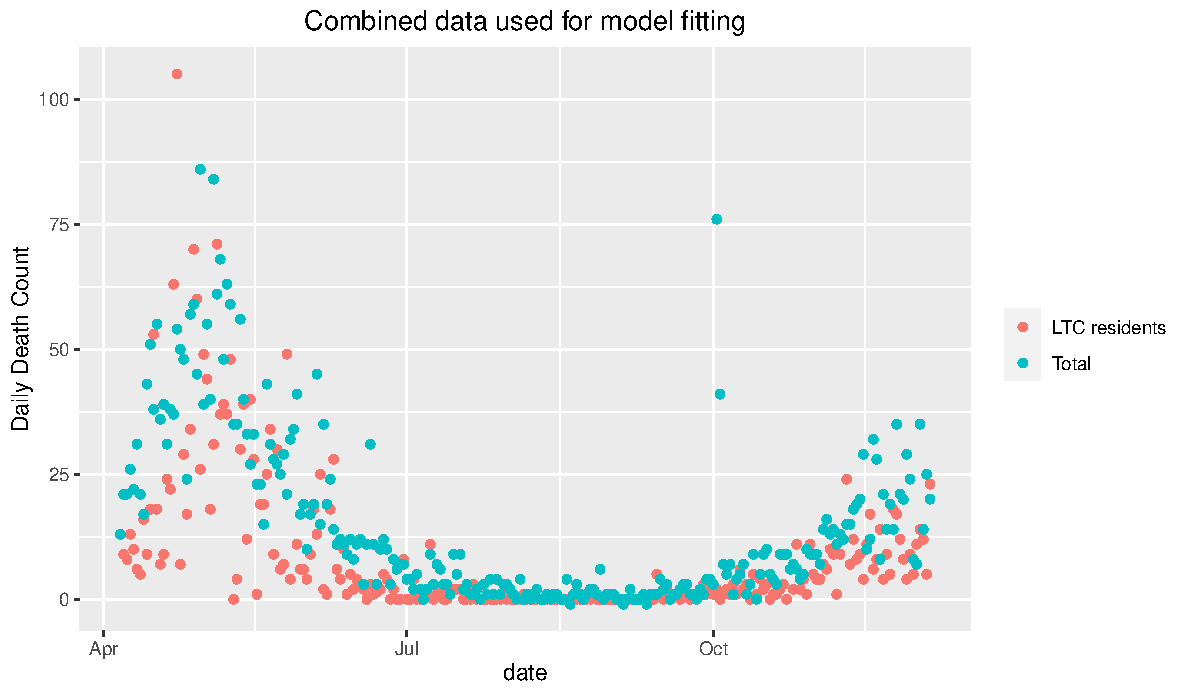
\includegraphics[scale = 0.7]{plot_combined_data.pdf}
    \caption{Combined data set obtained from multiple sources we used \label{figure: data} }\label{fig:foobar}
\end{figure}

\subsection{Data Sources}
The data set is composed from three different sources, which are
the daily cumulative death number in Ontario due to CoViD-19 given
in \cite{cite1}; the cumulative death number in LTC homes due to CoViD given in
\cite{cite2}; the daily death number obtained from daily CoViD report published
by the Ontario government. Then, by taking the lag difference in the cumulative
data sets we obtained the daily death number; finally, daily death number of
non-LTC residents are obtained by taking the difference between the total daily death number and LTC residents death number due to CoViD-19.

\subsection{Data Cleaning}
The source data sets used have the problem of incompleteness and inconsistencies. Daily death count in LTC homes prior to
April $25^{\text{th}}$ is not given in \cite{cite2}, so such information is obtained from cite3. Notwithstanding possible inconsistencies
introduced by composing two sources, daily death count in LTC homes in April is of critical importance for the understanding of first
wave of pandemic outbreak in Canada; therefore, such data cleaning procedure is justified.

Data publishers often correct their result in the latest data count without changing the errors in the previous published data, so we have
encountered negative daily death number when using lag difference on the cumulative data set $(n = 3)$; such negative death counts are replaced
by the mean of the death counts in two consecutive dates.

The daily death count of people not in LTC homes are obtained by taking difference between data from multiple sources, which also introduced negative
count numbers $(n =40)$; we tried to treat them as $0$ and missing, the difference in the resulting model is discussed in the section \ref{sec: results}.

The daily death count of people not in LTC homes on October $2 ^{\text{nd}}$ and $3^{\text{rd}}$ are found to be $74$ and $41$ respectively, which are considered to be outliers
and hence removed for model fitting.


\section{Methods}
In this study, we will use generalized addictive model (GAM) to model CoViD death data, which
will be introduced in this section.


\subsection{Negative Binomial GAM Model}


Let $Y_{i,t}$ be the number of death in $\mathcal P_\ltc$ and $\mathcal P_\ltc^C$ for $i =0,1$ respectively. It's a common to model the daily death count using Poisson model, but we do not  assume that the variance and mean are the same in our death data, hence a negative binomial model is used.

We assume $Y_{i,t}$ has the following hierarchical structure:
\begin{equation}
    \begin{array}{rcl} \label{eqn: model}
        Y_{i,t} &\sim& \mathrm{NB}(\lambda_{i,t}, \kappa)
        \\
        \log(\lambda_{i,t}) &=& \mu + I_{i=0} \beta_1 + U_i(t;\alpha_i),        
    \end{array}
\end{equation}
where $U_i$ are the non-parametric smoothing functions that are estimated using \verb|MGCV| package \cite{wood2015package};
$\kappa, \mu, \lambda_{i,t}, \beta_1, \alpha_i$ are unknown parameters estimated using maximum likelihood method.

In the model \eqref{eqn: model}, the parameter $\lambda_{1,t}$ and $\lambda_{0,t}$ described the daily death rate in $\mathcal{P}_\ltc$ and $\mathcal P_\ltc^C$ at time $t$. 
We assume at any fixed time $t_0$, the death rate in two subpopulation is roughly differed by a scalar factor due to epidemiological characteristic difference and is captured by the parameter $\beta_1$ and the difference between $U_1$ and $U_0$.


% % should we put the label in the LTC 
% \subsection{Model 2 - With the average cases of previous week}
% Model 2 is similar to model 1 except we add the average cases of previous week as the offset term.
% \begin{align}
% Y_{i,t} &\sim \mathrm{NB}(O_{i,t}\lambda_{i,t}, k) \label{model gam}
% \\
% \log(\lambda_{i,t}) &= \mu_i + I_{i=0} \beta_i + U_i(t;\alpha_i),
% \end{align}


\section{Results and Discussions \label{sec: results}} 
\subsection{Results}
Let $D_1(t)$ and $D_2(t)$ be the time series of death count in $\mathcal P_\ltc$ and $\mathcal P_\ltc^C$ respectively. To examine our hypothesis $H_0$, We fit the model \eqref{eqn: model} with \verb|gam| function in \verb|MGCV| \cite{wood2015package} and summarized the fitted daily death time series
$D_1$ and $D_2$ in Figure \ref{figure:model}.

As can be seen from Figure\ref{figure:model},
both time series have similar pattern with respect to time: both $D_1$ and $D_2$ reached a peak at May, had a relative flat curve during August to October and started to increase again after September.
However, deaths of the first outbreak between April and June most came from $\mathcal P_\ltc$ but this is not true for the second outbreak starting from October.

To further examine $H_0$, we have plotted the normalized difference of fitted time series $D_1$ and $D_2$ after the  log transformation and summarized in Figure \ref{fig: log diff}. It is clear from Figure \ref{fig: log diff} that $\log(D_1) - \log(D_2)$ is not a constant time series.

We remark that $D_1$ and $D_2$ are similar in scale, which implies the mortality rate of $\mathcal P_\ltc$ is much higher than that of $\mathcal P_\ltc^C$ due to difference in the population size, and this is consistent with the results obtained from other studies\cite{d2020coronavirus}.



\begin{figure}
    \centering
    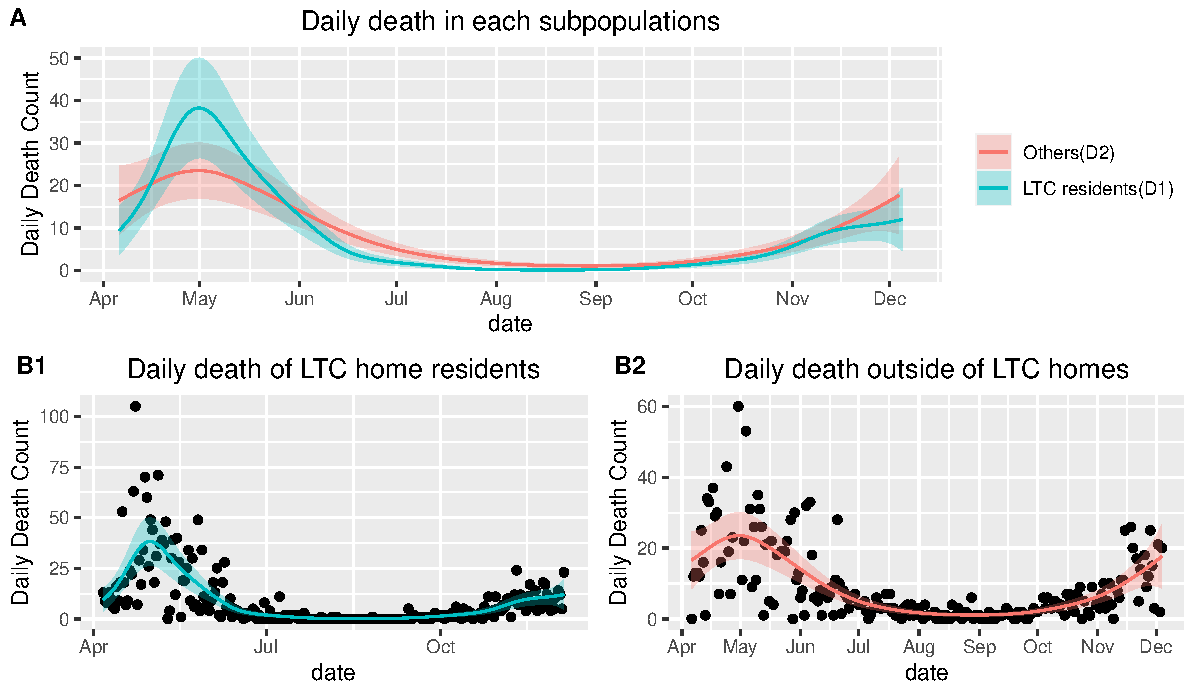
\includegraphics[scale = 0.8]{plot_model.pdf}
    \caption[]{
    Fitted $D_1$ and $D_2$ using Gam model. Fitted time series is plotted using solid line with
    shaded confidence interval.
        \par {\small
        \textbf{A}: Fitted $D_1$ and $D_2$ with confidence interval \label{figure:model} \\ 
        \textbf{B1}, \textbf{B2}: Fitted $D_1$ and $D_2$ with observed data in $\mathcal P_\ltc$ and $\mathcal P_\ltc^C$ as a reference.}
        }
\end{figure}
% 


\begin{figure}
    \centering
    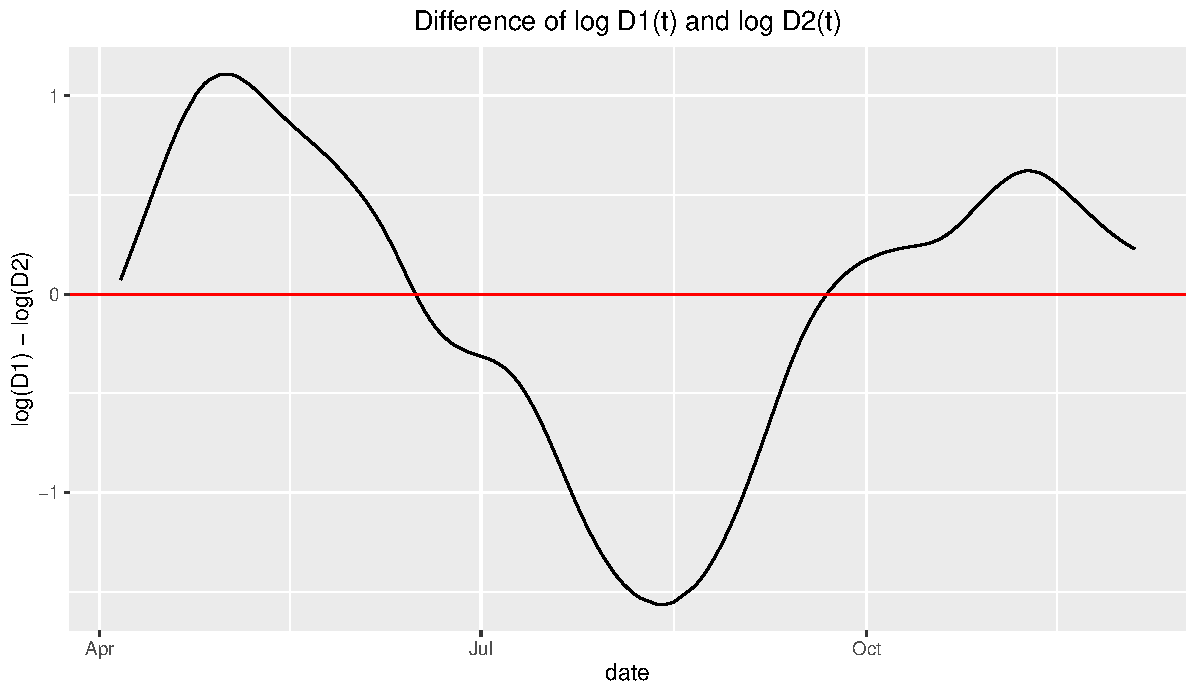
\includegraphics[scale = 0.7]{log_dif.pdf}
    \caption{The normalized difference between $\log(\widehat D_1)$ and $\log(\widehat D_2)$, where $\widehat D_1$ and $\widehat D_2$ are fitted time series using model \eqref{eqn: model}. Note that
    we have normalized the difference so the plotted time series is centered at $0$
     \label{fig: log diff}
    }
\end{figure}

\subsection{Discussions}

% \subsection{Results 2 - With average cases of previous week}
% \begin{figure}
%     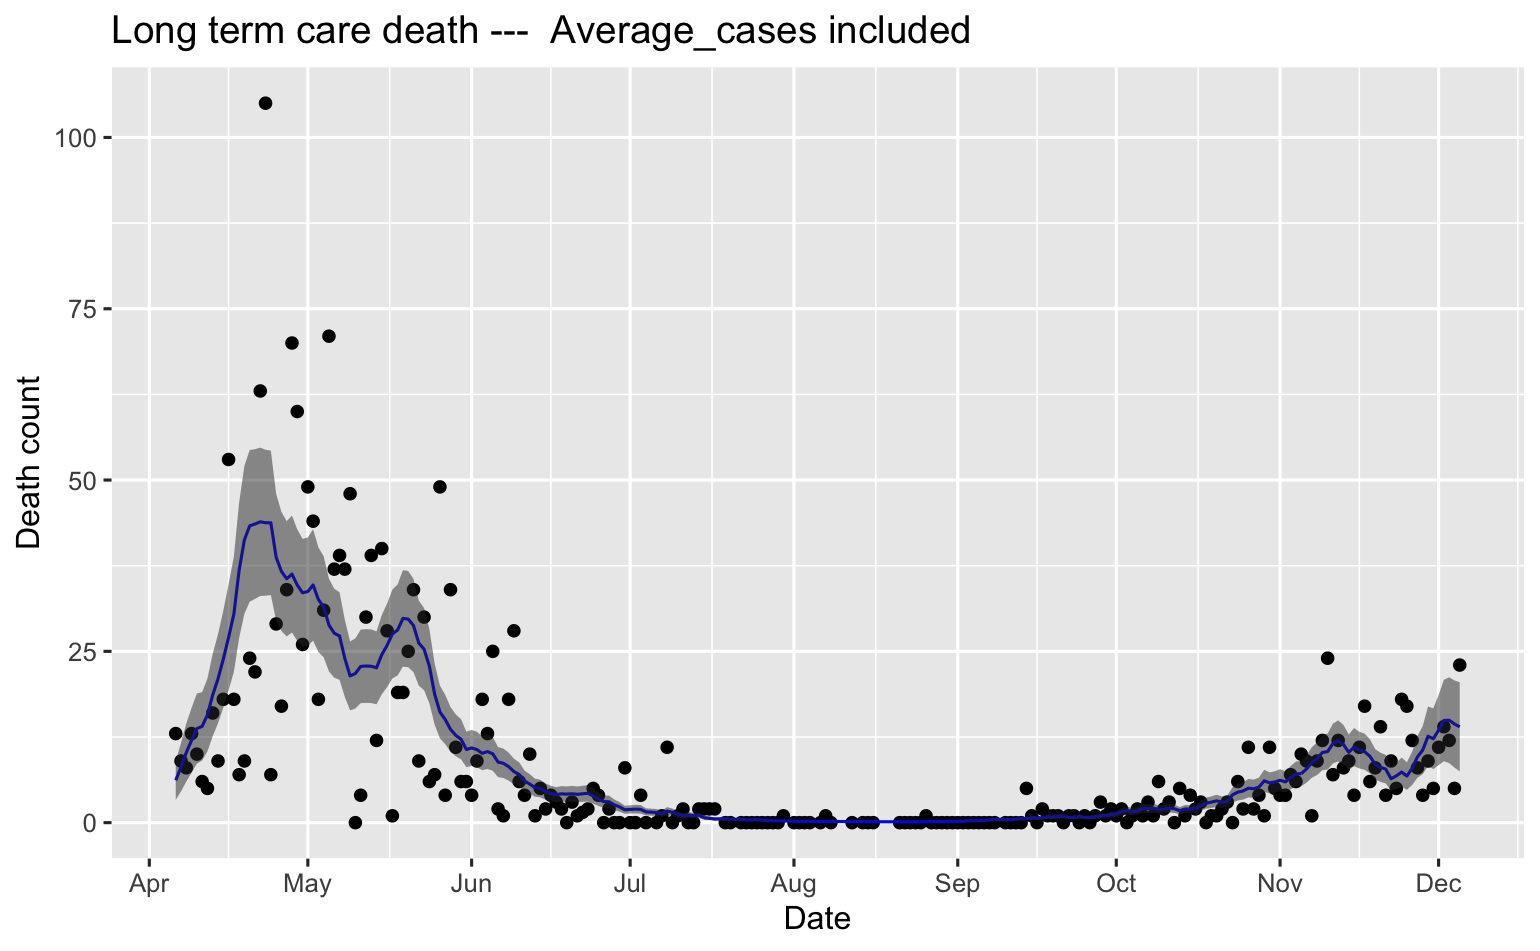
\includegraphics[width=0.55\textwidth]{ltc_with_average_cases.png}
%     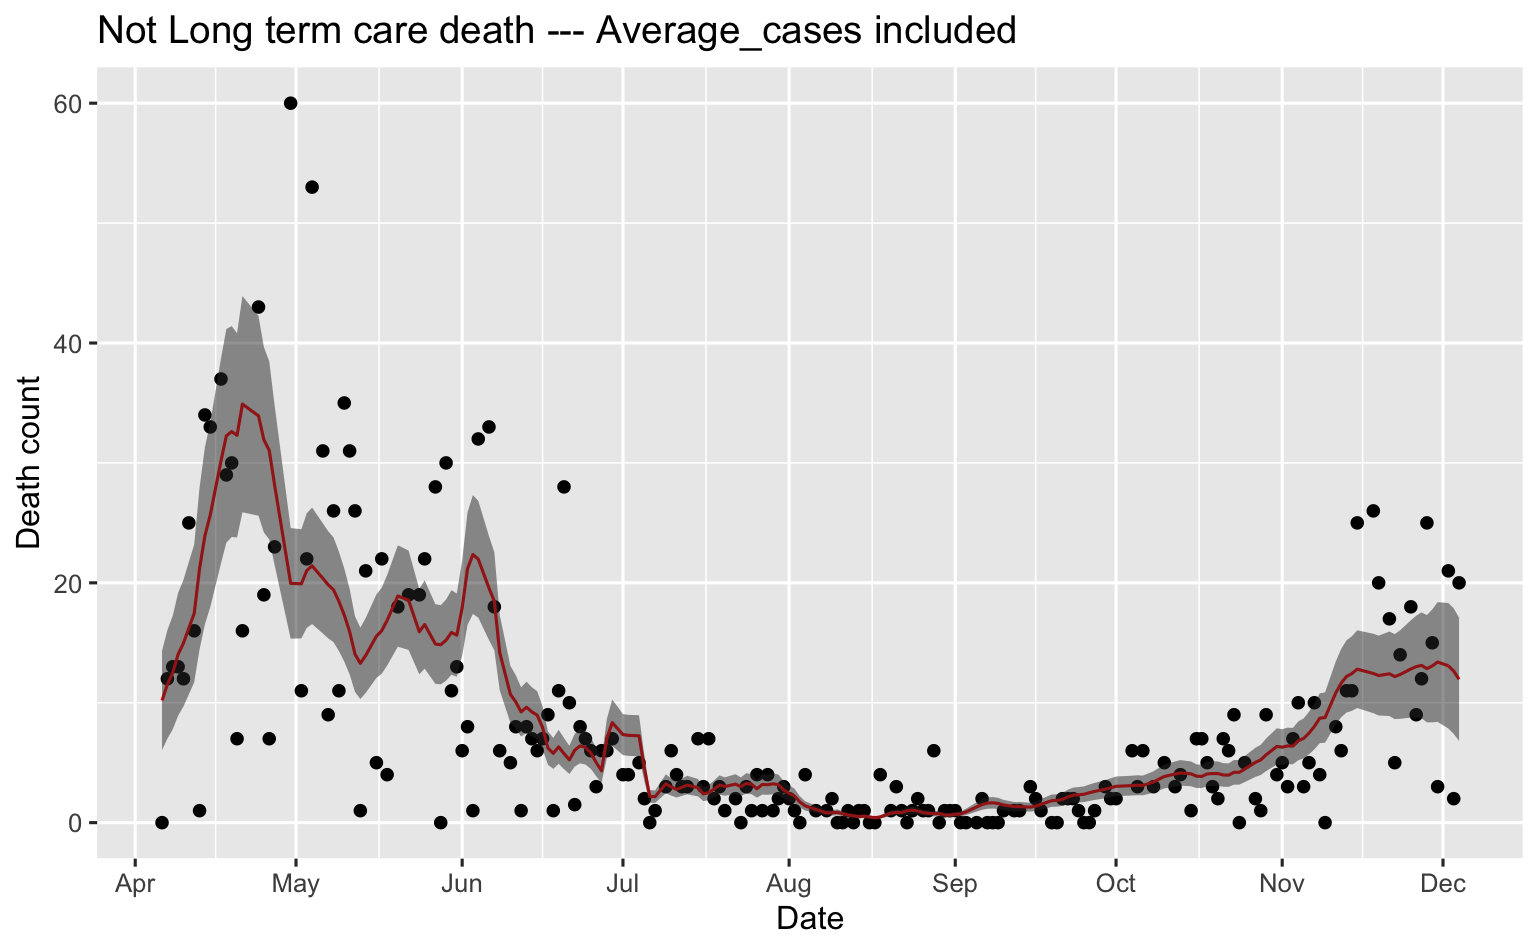
\includegraphics[width=0.55\textwidth]{non_ltc_with_average_cases.png}\\
%     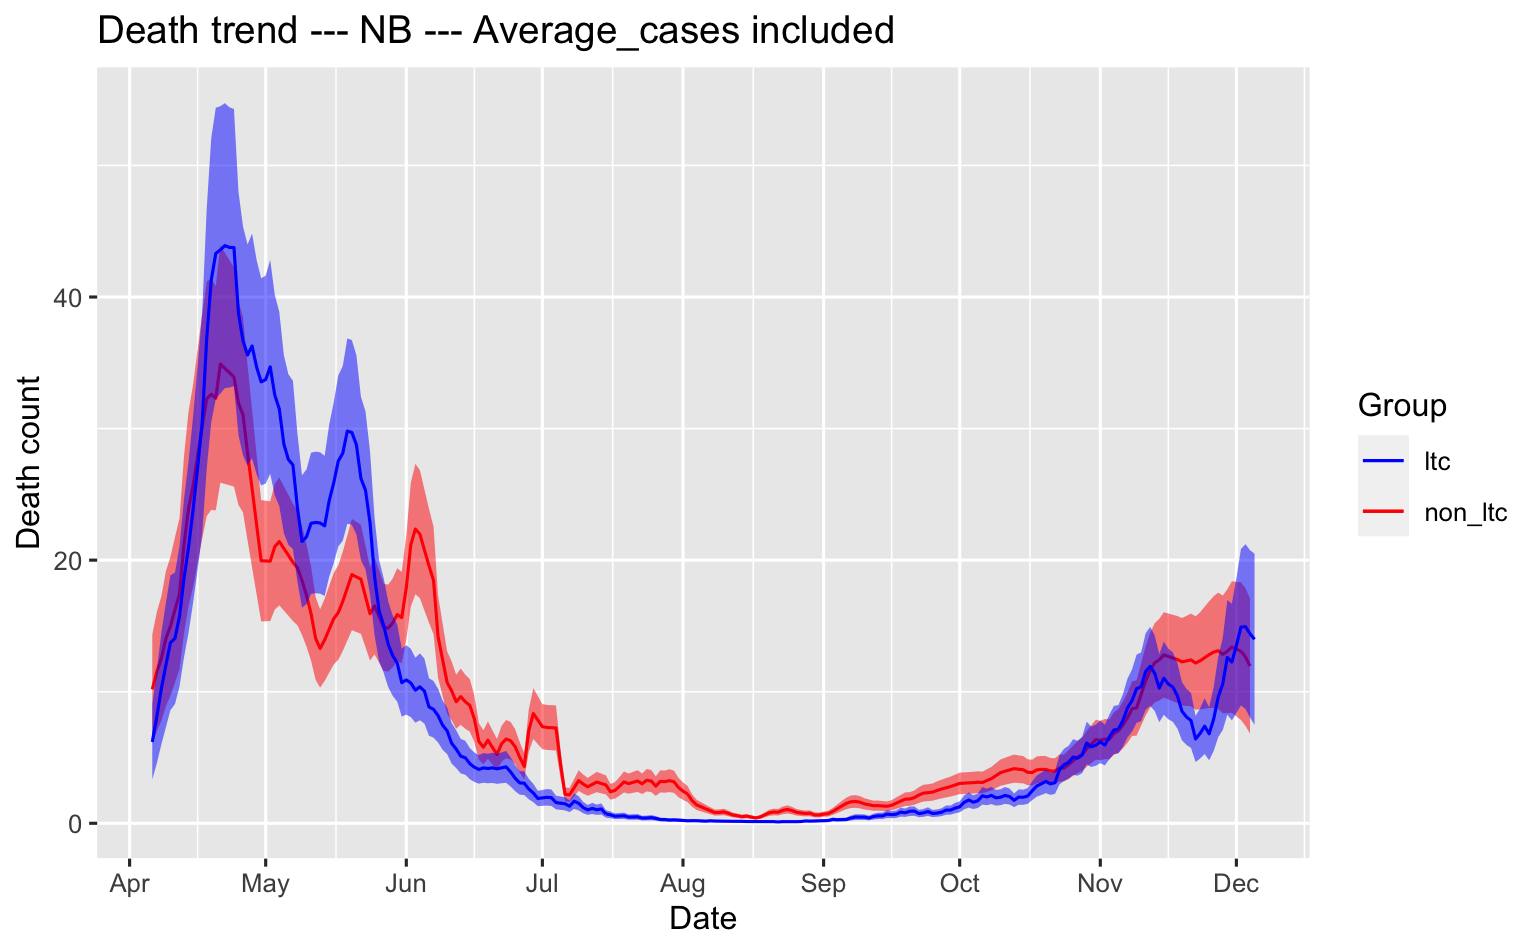
\includegraphics[width=1\textwidth]{two_trends_with_average_cases.png}
%     \caption{Model 2}\label{fig:foobar}
% \end{figure}

\subsubsection{Evidence Against $H_0$}
Under $H_0$, the ratio time series $D_1(t)/D_2(t)$ time series would be a constant, if we reasonably assume
the epidemiological characteristic of $\mathcal P_\ltc$ and $\mathcal P_\ltc^C$ does not change over time.
It can be seen from Figure \ref{figure:model} \textbf{A} and Figure \ref{fig: log diff} that $H_0$ can not be true. In particular, if $H_0$ is true, we would have observed a horizontal line around $y =0$ in Figure \ref{fig: log diff}.
So, we conclude that, there are two outbreaks occurred at different times, in the different subpopulations $\mathcal P_\ltc$ and $\mathcal P_\ltc^C$.

\subsubsection{Suggestions for Policy Makers}
By noting outbreaks occur in different subpopulations, some important implications and suggestions can be made for policy makers.
One should be careful when estimating the mortality rate of CoViD-19, since outbreaks in different time may occur
in the different subpopulations, then the estimated mortality rate from the historical data may not be a good predictor for future outbreaks.

For the reopening process in the future, restrictions on facilities with high risk population like schools and nursing home may be extended to reduce the chance and costs of outbreaks in such population. Finally, by closely monitoring and vaccinating the critical subpopulations like children in the day care and residents in the nursing home, we may effectively control the scale of the outbreak in the whole population. 
 
 We further remark that, multiple government agencies are publishing similar but incomplete and often conflicting data about CoViD-19, which jeopardized practical researches on the pandemic, as has pointed out in \cite{liu2020covid} and \cite{hsu2020understanding}. Hence, we urge the government to ensure departmental and interdepartmental communication so that a more consistent and comprehensive data source will be available for future researches.


\subsubsection{Limitations}
Despite its significance, our study have some major limitations. 
The final data set used is composed from multiple sources, which introduced a lot of inconsistencies besides the errors presented in each source. In particular,
the daily death counts of $\mathcal P_\ltc$ in April are obtained from daily reports \cite{cite2} published and are more error-prone than other sources for two reasons: the short time between obtaining and publishing data for the data publisher makes it difficult to check and correct mistakes; data publisher would not correct published daily report, since mistakes can be corrected in the future report.


The generalized addictive model is used to model the time series $D_1$ and $D_2$, which is a trade off between explainability and flexibility.  
Gam models are semi-parametric, so it's more susceptible to overfit the observed data than the parametric model. Overfitting might be eased with Jackknife method; we did not do so since forecasting is not of the central purpose of our model. 

Our model assumed the death rate in $\mathcal P_\ltc$ and $\mathcal P \ltc^C$ on average is different by a factor of $\exp{\beta_1}$, which is a fixed parameter to be estimated. However, $\mathcal P \ltc$ and $\mathcal P \ltc^C$ are vastly different in population size and so $\beta_1$ are difficult to interpret.

\subsubsection{Future Work}
Our method can be generalized in several ways. We have restricted ourselves to the pandemic occurs in Ontario, but similar method can be applied to the data for other regions and a comparison 
study may be conducted. In our model, the time series $D_1$ and $D_2$ does not explicitly depend on each other, which might not be realistic, so for future work a model incorporate the knowledge of corresponding subpopulations can be used. Since residents in LTC homes are often of high risk of CoViD-19, so future study can incorporate information such as age and social economic status in the model to reduce the possible confounding effect.










\newpage
%\bibliographystyle{unsrt}
\bibliographystyle{IEEEtran}

\bibliography{ref}
\end{document}